% answers.tex —— 2016 年·北京卷·文科 · 参考答案与详细解析片段
% 由 tools/generate_projects.py 依来源总账自 2016/2016_数学真题_北京文_试题.md + 2016/2016_数学真题_北京文_解析正文.md + 2016/2016_数学真题_北京文_答案要点.md 生成，勿手改（改源 MD 后重跑）


\begin{gktip}
固定原卷不附官方答案。以下为独立推导并经异人盲核对照的解析（非官方答案，等级 D）。第 8 题按「两个单项决赛名额相同、均为 8 人」理解作答：原卷仅给出立定跳远决赛人数，未明写跳绳决赛人数；该约定下结论唯一，且其余选项在任何取值下均可被反例排除。第 17 题直方图最左组 \([0,0.5)\) 的频率为 \(0\) 系原图如此（柱高之和恰为 \(1\) 可自证）。
\end{gktip}

\begin{answer}
\gksolhead{1}{}

\textbf{题目}：

已知集合 \(A=\{x\mid 2<x<4\}\)，\(B=\{x\mid x<3\) 或 \(x>5\}\)，则 \(A\cap B=\)（　）

（A）\(\{x\mid 2<x<5\}\)　（B）\(\{x\mid x<4\) 或 \(x>5\}\)

（C）\(\{x\mid 2<x<3\}\)　（D）\(\{x\mid x<2\) 或 \(x>5\}\)

\Needspace{4\baselineskip}
\textbf{解析}

\(A=(2,4)\)，\(B=(-\infty,3)\cup(5,+\infty)\)。在 \(A\) 内取同时属于 \(B\) 的部分：与 \((-\infty,3)\) 相交得 \((2,3)\)，与 \((5,+\infty)\) 无交，故 \(A\cap B=\{x\mid 2<x<3\}\)。

\gkanswer{答案：C，\(\{x\mid 2<x<3\}\)}

\end{answer}
\begin{answer}
\gksolhead{2}{}

\textbf{题目}：

复数 \(\dfrac{1+2\mathrm{i}}{2-\mathrm{i}}=\)（　）

\begin{gkopts}(2)
\task （A）\(\mathrm{i}\)
\task （B）\(1+\mathrm{i}\)
\task （C）\(-\mathrm{i}\)
\task （D）\(1-\mathrm{i}\)
\end{gkopts}

\Needspace{4\baselineskip}
\textbf{解析}

分母实数化：\(\dfrac{1+2\mathrm{i}}{2-\mathrm{i}}=\dfrac{(1+2\mathrm{i})(2+\mathrm{i})}{(2-\mathrm{i})(2+\mathrm{i})}=\dfrac{2+\mathrm{i}+4\mathrm{i}+2\mathrm{i}^2}{5}=\dfrac{5\mathrm{i}}{5}=\mathrm{i}\)。

\gkanswer{答案：A，\(\mathrm{i}\)}

\end{answer}
\begin{answer}
\gksolhead{3}{}

\textbf{题目}：

执行如图所示的程序框图，输出的 \(s\) 值为（　）
\nopagebreak[4]
\begin{center}% 第 3 题程序框图：按固定源 PDF 的框图结构逐一重绘（框形、分支标签与回边走向照原图）。
% 回边次序（易错点，600 dpi 逐箭头核对）：「是」分支先进入 \(s=s+k^{3}\)（箭头指向其下沿），
% 再上行进入 \(k=k+1\)，最后由 \(k=k+1\) 顶边折回主干，箭头指向主干（T 形汇入）。
% 坐标全部显式给定：主干 x=0；回边列 x=-3.4；join 在 init 底边下 0.35cm；
% inc 顶边(-2.6) 与 init 底边(-1.4) 留 1.2cm 空档，杜绝框体重叠与回边穿框。
\begin{tikzpicture}[>=stealth,every node/.style={font=\small},
  term/.style={draw,rounded corners,minimum width=1.5cm,minimum height=6mm},
  box/.style={draw,minimum width=2.2cm,minimum height=6mm},
  io/.style={draw,trapezium,trapezium left angle=70,trapezium right angle=110,minimum width=1.9cm,minimum height=6mm},
  decision/.style={draw,diamond,aspect=2.6,minimum width=2.6cm,minimum height=1.0cm,inner sep=0pt}]
\node[term] (start) at (0,0) {开始};
\node[box] (init) at (0,-1.1) {\(k=0,\ s=0\)};
\node[decision] (test) at (0,-6.6) {\(k\leqslant 2\)};
\node[io] (out) at (0,-8.0) {输出 \(s\)};
\node[term] (end) at (0,-9.2) {结束};
\node[box] (inc) at (-3.4,-2.9) {\(k=k+1\)};
\node[box] (add) at (-3.4,-4.5) {\(s=s+k^{3}\)};
\coordinate (join) at (0,-1.75);
\draw[->] (start)--(init);
\draw[->] (init)--(test);
\draw[->] (test.south)--node[right,xshift=2pt]{否}(out.north);
\draw[->] (out)--(end);
\draw[->] (test.west) -| node[above,pos=0.35]{是} (add.south);
\draw[->] (add.north)--(inc.south);
\draw[->] (inc.north) |- (join);
\end{tikzpicture}
\end{center}
\nopagebreak[4]
\begin{gkopts}(2)
\task （A）\(8\)
\task （B）\(9\)
\task （C）\(27\)
\task （D）\(36\)
\end{gkopts}

\Needspace{4\baselineskip}
\textbf{解析}

框图回边的次序为：判断框「\(k\leqslant2\)」为「是」时\textbf{先}执行 \(s=s+k^{3}\)，\textbf{再}执行 \(k=k+1\)，然后回到判断。初始 \(k=0\)，\(s=0\)：

\begin{itemize}
\item \(k=0\)：\(0\leqslant2\)，\(s=0+0^{3}=0\)，\(k=1\)；
\item \(k=1\)：\(1\leqslant2\)，\(s=0+1^{3}=1\)，\(k=2\)；
\item \(k=2\)：\(2\leqslant2\)，\(s=1+2^{3}=9\)，\(k=3\)；
\item \(k=3\)：\(3\leqslant2\) 不成立，输出 \(s=9\)。
\end{itemize}

故输出的 \(s\) 值为 \(9\)（累加的是 \(0^{3}+1^{3}+2^{3}\)；若误按「先自增」读将得 \(36\)，与框图箭头次序不符）。

\gkanswer{答案：B，\(9\)}

\end{answer}
\begin{answer}
\gksolhead{4}{}

\textbf{题目}：

下列函数中，在区间 \((-1,1)\) 上为减函数的是（　）

\begin{gkopts}(2)
\task （A）\(y=\dfrac{1}{1-x}\)
\task （B）\(y=\cos x\)
\task （C）\(y=\ln(x+1)\)
\task （D）\(y=2^{-x}\)
\end{gkopts}

\Needspace{4\baselineskip}
\textbf{解析}

（A）\(y'=\dfrac{1}{(1-x)^{2}}>0\)，在 \((-1,1)\) 上递增；（B）\(y=\cos x\) 在 \((-1,1)\) 上先增后减，不单调；（C）\(y'=\dfrac{1}{x+1}>0\)（\(x>-1\)），递增；（D）\(y=2^{-x}=\left(\dfrac12\right)^x\)，底数小于 \(1\)，在 \(\mathbf{R}\) 上单调递减。故选（D）。

\gkanswer{答案：D，\(y=2^{-x}\)}

\end{answer}
\begin{answer}
\gksolhead{5}{}

\textbf{题目}：

圆 \((x+1)^{2}+y^{2}=2\) 的圆心到直线 \(y=x+3\) 的距离为（　）

\begin{gkopts}(2)
\task （A）\(1\)
\task （B）\(2\)
\task （C）\(\sqrt{2}\)
\task （D）\(2\sqrt{2}\)
\end{gkopts}

\Needspace{4\baselineskip}
\textbf{解析}

\Needspace{5\baselineskip}
圆心为 \((-1,0)\)。直线 \(y=x+3\) 即 \(x-y+3=0\)，圆心到它的距离

\nopagebreak[4]
\[
d=\frac{|(-1)-0+3|}{\sqrt{1^{2}+(-1)^{2}}}=\frac{2}{\sqrt{2}}=\sqrt{2}.
\]

（恰等于半径，直线与圆相切，可作旁证。）

\gkanswer{答案：C，\(\sqrt{2}\)}

\end{answer}
\begin{answer}
\gksolhead{6}{}

\textbf{题目}：

从甲、乙等 \(5\) 名学生中随机选出 \(2\) 人，则甲被选中的概率为（　）

\begin{gkopts}(2)
\task （A）\(\dfrac{1}{5}\)
\task （B）\(\dfrac{2}{5}\)
\task （C）\(\dfrac{8}{25}\)
\task （D）\(\dfrac{9}{25}\)
\end{gkopts}

\Needspace{4\baselineskip}
\textbf{解析}

从 \(5\) 人中任选 \(2\) 人共有 \(\mathrm C_5^2=10\) 种等可能结果；甲被选中的结果有 \(\mathrm C_4^1=4\) 种，故概率为 \(\dfrac{4}{10}=\dfrac{2}{5}\)。

\gkanswer{答案：B，\(\dfrac{2}{5}\)}

\end{answer}
\begin{answer}
\gksolhead{7}{}

\textbf{题目}：

已知 \(A(2,5)\)，\(B(4,1)\)。若点 \(P(x,y)\) 在线段 \(AB\) 上，则 \(2x-y\) 的最大值为（　）

\begin{gkopts}(2)
\task （A）\(-1\)
\task （B）\(3\)
\task （C）\(7\)
\task （D）\(8\)
\end{gkopts}

\Needspace{4\baselineskip}
\textbf{解析}

\Needspace{5\baselineskip}
设 \(P=(2,5)+t\big((4,1)-(2,5)\big)=(2+2t,\ 5-4t)\)，\(t\in[0,1]\)。则

\nopagebreak[4]
\[
2x-y=2(2+2t)-(5-4t)=8t-1,
\]

关于 \(t\) 递增，在 \(t=1\)（即 \(P=B\)）处取最大值 \(7\)。

\gkanswer{答案：C，\(7\)}

\end{answer}
\begin{answer}
\gksolhead{8}{}

\textbf{题目}：

某学校运动会的立定跳远和 \(30\) 秒跳绳两个单项比赛分成预赛和决赛两个阶段，下表为 \(10\) 名学生的预赛成绩，其中有三个数据模糊。

\begin{center}
\begin{tabular}{llllll}
\toprule
学生序号 & \(1\) & \(2\) & \(3\) & \(4\) & \(5\) \\
\midrule
立定跳远（单位：米） & \(1.96\) & \(1.92\) & \(1.82\) & \(1.80\) & \(1.78\) \\
\(30\) 秒跳绳（单位：次） & \(63\) & \(a\) & \(75\) & \(60\) & \(63\) \\
学生序号 & \(6\) & \(7\) & \(8\) & \(9\) & \(10\) \\
立定跳远（单位：米） & \(1.76\) & \(1.74\) & \(1.72\) & \(1.68\) & \(1.60\) \\
\(30\) 秒跳绳（单位：次） & \(72\) & \(70\) & \(a-1\) & \(b\) & \(65\) \\
\bottomrule
\end{tabular}
\end{center}

在这 \(10\) 名学生中，进入立定跳远决赛的有 \(8\) 人，同时进入立定跳远决赛和 \(30\) 秒跳绳决赛的有 \(6\) 人，则（　）

（A）\(2\) 号学生进入 \(30\) 秒跳绳决赛　（B）\(5\) 号学生进入 \(30\) 秒跳绳决赛

（C）\(8\) 号学生进入 \(30\) 秒跳绳决赛　（D）\(9\) 号学生进入 \(30\) 秒跳绳决赛

\Needspace{4\baselineskip}
\textbf{解析}

立定跳远的 \(10\) 个成绩互不相同且按序号递减，故进入立定跳远决赛的 \(8\) 人恰为 \(1\)—\(8\) 号，\(9\)、\(10\) 号未进该项决赛。

原卷只明确跳远决赛有 8 人，未明确跳绳决赛人数，不能据两个项目均设预赛和决赛推断名额相同。本题答案待核（ISSUE-1005）。

反例：取 \(a=55\)、\(b=50\)，跳绳成绩从高到低为 3、6、7、10、1 与 5（同分）、4、2、8、9 号。若跳绳决赛取前 7 人，则入选集合为 \(\{1,3,4,5,6,7,10\}\)，与跳远入选的 1—8 号恰有 6 人重合，满足已知条件，却使 9 号不入选。这说明 D 并非现有题面必然结论。

仅在获得可靠来源确认两项目决赛均为 8 人后，才能推导：跳绳入选者中 6 人来自 1—8 号，其余两席只能是 9、10 号，因此选 D。当前不擅自补入该条件，保留待核。

\gkanswer{答案：U}

\end{answer}
\begin{answer}
\gksolhead{9}{}

\textbf{题目}：

已知向量 \(\boldsymbol{a}=(1,\sqrt{3})\)，\(\boldsymbol{b}=(\sqrt{3},1)\) 则 \(\boldsymbol{a}\) 与 \(\boldsymbol{b}\) 夹角的大小为 \(\underline{\qquad}\)。

\Needspace{4\baselineskip}
\textbf{解析}

\Needspace{5\baselineskip}
\(\boldsymbol{a}\cdot\boldsymbol{b}=1\times\sqrt{3}+\sqrt{3}\times1=2\sqrt{3}\)，\(|\boldsymbol{a}|=|\boldsymbol{b}|=2\)。设夹角为 \(\theta\)，则

\nopagebreak[4]
\[
\cos\theta=\frac{\boldsymbol{a}\cdot\boldsymbol{b}}{|\boldsymbol{a}||\boldsymbol{b}|}=\frac{2\sqrt{3}}{4}=\frac{\sqrt{3}}{2},
\]

由 \(\theta\in[0,\pi]\) 得 \(\theta=\dfrac{\pi}{6}\)。

\gkanswer{答案：\(\dfrac{\pi}{6}\)}

\end{answer}
\begin{answer}
\gksolhead{10}{}

\textbf{题目}：

函数 \(f(x)=\dfrac{x}{x-1}\)（\(x\geqslant 2\)）的最大值为 \(\underline{\qquad}\)。

\Needspace{4\baselineskip}
\textbf{解析}

\(f(x)=\dfrac{x}{x-1}=1+\dfrac{1}{x-1}\)。在 \(x\geqslant2\) 上 \(x-1\geqslant1\)，\(\dfrac{1}{x-1}\) 随 \(x\) 增大而减小（取值落在 \((0,1]\)），故 \(f\) 在 \([2,+\infty)\) 上递减，最大值在 \(x=2\) 处取得：\(f(2)=2\)。

\gkanswer{答案：\(2\)}

\end{answer}
\begin{answer}
\gksolhead{11}{}

\textbf{题目}：

某四棱柱的三视图如图所示，则该四棱柱的体积为 \(\underline{\qquad}\)。
\nopagebreak[4]
\begin{center}% 第 11 题四棱柱三视图：按固定源 PDF 的视图排布与尺寸线位置重绘（数字只保留原图印出的 1、1、1、2）。
% 正（主）视图为 2:1 矩形、内部两条竖直虚线在宽度的 1/4 与 3/4 处（梯形两斜棱的投影），原图无尺寸标注。
% 俯视图整块较视图标签下移 0.5cm：标签（锚 y=-0.32，字高约 0.37）与上底尺寸线（y=-1.12）留出 0.43cm 白隙。
\begin{tikzpicture}[every node/.style={font=\small},scale=0.9,line cap=round,line join=round]
% 正（主）视图：矩形内两条竖直虚线，无尺寸标注
\draw (0,0) rectangle (2.0,1.0);
\draw[dashed] (0.5,0)--(0.5,1.0);
\draw[dashed] (1.5,0)--(1.5,1.0);
\node[below] at (1.0,-0.32) {正（主）视图};
% 侧（左）视图：正方形；右侧竖直尺寸线（两端端线），数字 1 在旁
\draw (3.3,0) rectangle (4.3,1.0);
\draw[<->] (4.68,0)--(4.68,1.0);
\draw (4.55,0)--(4.81,0); \draw (4.55,1.0)--(4.81,1.0);
\node[right] at (4.85,0.5) {\(1\)};
\node[below] at (3.8,-0.32) {侧（左）视图};
% 俯视图：等腰梯形（上底 1、下底 2、高 1）；上底上方数字 1 断开的水平尺寸线，
% 右侧竖直尺寸线旁标 1，下底下方数字 2 断开的水平尺寸线
\draw (0,-2.4)--(2.0,-2.4)--(1.5,-1.4)--(0.5,-1.4)--cycle;
\draw[<->] (0.5,-1.12)--(1.5,-1.12);
\node[fill=white,inner sep=1.2pt] at (1.0,-1.12) {\(1\)};
\draw[<->] (2.42,-1.4)--(2.42,-2.4);
\draw (2.29,-1.4)--(2.55,-1.4); \draw (2.29,-2.4)--(2.55,-2.4);
\node[right] at (2.58,-1.9) {\(1\)};
\draw[<->] (0,-2.68)--(2.0,-2.68);
\node[fill=white,inner sep=1.2pt] at (1.0,-2.68) {\(2\)};
\node[below] at (1.0,-3.05) {俯视图};
\end{tikzpicture}
\end{center}
\nopagebreak[4]
\Needspace{4\baselineskip}
\textbf{解析}

\Needspace{5\baselineskip}
由俯视图，底面是上底 \(1\)、下底 \(2\)、两底间距离 \(1\) 的等腰梯形，面积

\nopagebreak[4]
\[
S=\frac{1+2}{2}\times1=\frac{3}{2}.
\]

\Needspace{5\baselineskip}
正（主）视图为 \(2\times1\) 的矩形（宽 \(2\) 即梯形下底，中间两条竖直虚线是梯形两斜棱的投影）、侧（左）视图为边长 \(1\) 的正方形，两者共同给出棱柱的高为 \(1\)。故体积

\nopagebreak[4]
\[
V=Sh=\frac{3}{2}\times1=\frac{3}{2}.
\]

\gkanswer{答案：\(\dfrac{3}{2}\)}

\end{answer}
\begin{answer}
\gksolhead{12}{}

\textbf{题目}：

已知双曲线 \(\dfrac{x^{2}}{a^{2}}-\dfrac{y^{2}}{b^{2}}=1\)（\(a>0\)，\(b>0\)）的一条渐近线为 \(2x+y=0\)，一个焦点为 \((\sqrt{5},0)\)，则 \(a=\underline{\qquad}\)；\(b=\underline{\qquad}\)。

\Needspace{4\baselineskip}
\textbf{解析}

\Needspace{5\baselineskip}
双曲线的渐近线为 \(y=\pm\dfrac{b}{a}x\)。由一条渐近线 \(2x+y=0\) 即 \(y=-2x\) 得 \(\dfrac{b}{a}=2\)，即 \(b=2a\)。焦点 \((\sqrt{5},0)\) 给出 \(c=\sqrt{5}\)，而 \(c^{2}=a^{2}+b^{2}\)，故

\nopagebreak[4]
\[
5=a^{2}+4a^{2}=5a^{2},
\]

得 \(a=1\)，从而 \(b=2\)。

\gkanswer{答案：\(a=1\)；\(b=2\)。}

\end{answer}
\begin{answer}
\gksolhead{13}{}

\textbf{题目}：

在 \(\triangle ABC\) 中，\(\angle A=\dfrac{2\pi}{3}\)，\(a=\sqrt{3}c\)，则 \(\dfrac{b}{c}=\underline{\qquad}\)。

\Needspace{4\baselineskip}
\textbf{解析}

\Needspace{5\baselineskip}
由正弦定理 \(\dfrac{a}{\sin A}=\dfrac{c}{\sin C}\)，得

\nopagebreak[4]
\[
\sin C=\frac{c}{a}\sin A=\frac{1}{\sqrt{3}}\times\frac{\sqrt{3}}{2}=\frac12 .
\]

故 \(C=\dfrac{\pi}{6}\) 或 \(C=\dfrac{5\pi}{6}\)；后者会使 \(A+C=\dfrac{2\pi}{3}+\dfrac{5\pi}{6}>\pi\)，舍去。取 \(C=\dfrac{\pi}{6}\)，则 \(B=\pi-\dfrac{2\pi}{3}-\dfrac{\pi}{6}=\dfrac{\pi}{6}=C\)，故 \(b=c\)，\(\dfrac{b}{c}=1\)。

\gkanswer{答案：\(1\)}

\end{answer}
\begin{answer}
\gksolhead{14}{}

\textbf{题目}：

某网店统计了连续三天售出商品的种类情况：第一天售出 \(19\) 种商品，第二天售出 \(13\) 种商品，第三天售出 \(18\) 种商品；前两天都售出的商品有 \(3\) 种，后两天都售出的商品有 \(4\) 种，则该网店

① 第一天售出但第二天未售出的商品有 \(\underline{\qquad}\) 种；

② 这三天售出的商品最少有 \(\underline{\qquad}\) 种。

\Needspace{4\baselineskip}
\textbf{解析}

\gksubpart{①}

第一天售出的 \(19\) 种中，与第二天重合的有 \(3\) 种，故第一天售出而第二天未售出的有 \(19-3=16\) 种。

\gksubpart{②}

\Needspace{5\baselineskip}
记三天售出商品的集合为 \(A\)、\(B\)、\(C\)，\(|A|=19\)，\(|B|=13\)，\(|C|=18\)，\(|A\cap B|=3\)，\(|B\cap C|=4\)。由

\nopagebreak[4]
\[
|A\cup B\cup C|=|A\cup B|+|C|-|C\cap(A\cup B)|,\qquad |A\cup B|=19+13-3=29,
\]

\Needspace{5\baselineskip}
要使总数最小，需使 \(|C\cap(A\cup B)|\) 最大。而

\nopagebreak[4]
\[
|C\cap(A\cup B)|=|A\cap C|+|B\cap C|-|A\cap B\cap C|
=|A\cap C|-|A\cap B\cap C|+4,
\]

其中 \(|A\cap C|-|A\cap B\cap C|=|(A\cap C)\setminus B|\leqslant|C\setminus B|=18-4=14\)，故 \(|C\cap(A\cup B)|\leqslant18\)，从而 \(|A\cup B\cup C|\geqslant29+18-18=29\)。

该下界可达：令 \(A\cap B\) 全部含于 \(C\)，且 \(C\setminus B\) 的 \(14\) 种全在 \(A\) 中，此时 \(|C\cap(A\cup B)|=18\)。故这三天售出的商品最少有 \(29\) 种。

\gkanswer{答案：① \(16\)；② \(29\)。}

\end{answer}
\begin{answer}
\gksolhead{15}{}

\textbf{题目}：

已知 \(\{a_{n}\}\) 是等差数列，\(\{b_{n}\}\) 是等比数列，且 \(b_{2}=3\)，\(b_{3}=9\)，\(a_{1}=b_{1}\)，\(a_{14}=b_{4}\)。

（1） 求 \(\{a_{n}\}\) 的通项公式；

（2） 设 \(c_{n}=a_{n}+b_{n}\)，求数列 \(\{c_{n}\}\) 的前 \(n\) 项和。

\Needspace{4\baselineskip}
\textbf{解析}

\gksubpart{(1)}

设等比数列 \(\{b_n\}\) 的公比为 \(q\)。由 \(b_2=3\)、\(b_3=9\) 相除得 \(q=3\)，代回得 \(b_1=1\)，故 \(b_4=27\)。

\Needspace{5\baselineskip}
于是 \(a_1=b_1=1\)，\(a_{14}=b_4=27\)。设等差数列公差为 \(d\)，由 \(a_{14}=a_1+13d\) 得 \(1+13d=27\)，\(d=2\)。故

\nopagebreak[4]
\[
a_n=1+2(n-1)=2n-1.
\]

\gksubpart{(2)}

\Needspace{5\baselineskip}
\(c_n=a_n+b_n=(2n-1)+3^{n-1}\)。前 \(n\) 项和拆为两部分：

\nopagebreak[4]
\[
\sum_{k=1}^{n}(2k-1)=n^{2},\qquad
\sum_{k=1}^{n}3^{k-1}=\frac{3^{n}-1}{3-1}=\frac{3^{n}-1}{2},
\]

\Needspace{5\baselineskip}
故

\nopagebreak[4]
\[
S_n=n^{2}+\frac{3^{n}-1}{2}.
\]

\gkanswer{答案（1）：\(a_n=2n-1\)。}

\gkanswer{答案（2）：\(S_n=n^{2}+\dfrac{3^{n}-1}{2}\)。}

\end{answer}
\begin{answer}
\gksolhead{16}{}

\textbf{题目}：

已知函数 \(f(x)=2\sin\omega x\cos\omega x+\cos 2\omega x\)（\(\omega>0\)）的最小正周期为 \(\pi\)。

（1） 求 \(\omega\) 的值；

（2） 求 \(f(x)\) 的单调递增区间。

\Needspace{4\baselineskip}
\textbf{解析}

\gksubpart{(1)}

\Needspace{5\baselineskip}
由二倍角公式 \(2\sin\omega x\cos\omega x=\sin 2\omega x\)，得

\nopagebreak[4]
\[
f(x)=\sin 2\omega x+\cos 2\omega x=\sqrt{2}\sin\left(2\omega x+\frac{\pi}{4}\right).
\]

最小正周期 \(T=\dfrac{2\pi}{2\omega}=\dfrac{\pi}{\omega}\)，由 \(T=\pi\) 得 \(\omega=1\)。

\gksubpart{(2)}

\Needspace{5\baselineskip}
此时 \(f(x)=\sqrt{2}\sin\left(2x+\dfrac{\pi}{4}\right)\)。正弦函数在 \(\left[-\dfrac{\pi}{2}+2k\pi,\ \dfrac{\pi}{2}+2k\pi\right]\) 上递增，故

\nopagebreak[4]
\[
-\frac{\pi}{2}+2k\pi\leqslant2x+\frac{\pi}{4}\leqslant\frac{\pi}{2}+2k\pi,
\]

\Needspace{5\baselineskip}
解得

\nopagebreak[4]
\[
-\frac{3\pi}{8}+k\pi\leqslant x\leqslant\frac{\pi}{8}+k\pi,
\]

即单调递增区间为 \(\left[k\pi-\dfrac{3\pi}{8},\ k\pi+\dfrac{\pi}{8}\right]\)（\(k\in\mathbf{Z}\)）。

\gkanswer{答案（1）：\(\omega=1\)。}

\gkanswer{答案（2）：\(\left[k\pi-\dfrac{3\pi}{8},\ k\pi+\dfrac{\pi}{8}\right]\)（\(k\in\mathbf{Z}\)）。}

\end{answer}
\begin{answer}
\gksolhead{17}{}

\textbf{题目}：

某市居民用水拟实行阶梯水价，每人每月用水量中不超过 \(w\) 立方米的部分按 \(4\) 元/立方米收费，超出 \(w\) 立方米的部分按 \(10\) 元/立方米收费，从该市随机调查了 \(10000\) 位居民，获得了他们某月的用水量数据，整理得到如图频率分布直方图：
\nopagebreak[4]
\begin{center}% 第 17 题频率分布直方图：柱高按固定源 PDF 像素实测重绘（组距 0.5，共 9 组）。
% 最左组 [0,0.5) 频率为 0（原图如此）：纵轴与第一根柱之间留一个组距空档，不画柱。
\begin{tikzpicture}[>=stealth,every node/.style={font=\small}]
\def\ux{1.15}   % 横轴：1 立方米
\def\uy{3.6}    % 纵轴：单位 1（频率/组距）
% 坐标轴（横轴标题置于轴箭头右端之后，与原图一致；不可用 below left 锚到 (5.45,0)——会覆盖 2.5–4.5 刻度）
\draw[->] (0,0)--(5.45,0) node[right,yshift=-2pt] {用水量（立方米）};
\draw[->] (0,0)--(0,2.05);
\node[anchor=south west] at (0.10,2.02) {\begin{tabular}{c}频率\\\hline 组距\end{tabular}};
% 刻度虚线（0.1–0.5）与纵轴刻度标签
\foreach \v in {0.1,0.2,0.3,0.4,0.5} {
  \draw[dashed] (0,\v*\uy)--(5.1,\v*\uy);
  \node[left] at (-0.08,\v*\uy) {\(\v\)};
}
% 横轴刻度标签
\foreach \t in {0,0.5,1,1.5,2,2.5,3,3.5,4,4.5} {
  \node[below] at (\t*\ux,-0.10) {\(\t\)};
}
% 柱（空心矩形，相邻柱共用竖边；最左组无柱）：
% [0.5,1)=0.2，[1,1.5)=0.3，[1.5,2)=0.4，[2,2.5)=0.5，[2.5,3)=0.3，[3,3.5)=[3.5,4)=[4,4.5)=0.1
\foreach \i/\h in {1/0.2, 2/0.3, 3/0.4, 4/0.5, 5/0.3, 6/0.1, 7/0.1, 8/0.1} {
  \draw ({0.5*\i*\ux},0) rectangle ({0.5*(\i+1)*\ux},{\h*\uy});
}
\end{tikzpicture}
\end{center}
\nopagebreak[4]
（1） 如果 \(w\) 为整数，那么根据此次调查，为使 80\% 以上居民在该月的用水价格为 \(4\) 元/立方米，\(w\) 至少定为多少？

（2） 假设同组中的每个数据用该组区间的右端点值代替，当 \(w=3\) 时，估计该市居民该月的人均水费。

\Needspace{4\baselineskip}
\textbf{解析}

\Needspace{5\baselineskip}
各组的组距均为 \(0.5\)。由直方图读出各组的频率 \(=\)（频率/组距）\(\times0.5\)：\((0,0.5]\) 与 \((0.5,1]\) 以外的各组依次为

\nopagebreak[4]
\[
0.1,\ 0.15,\ 0.2,\ 0.25,\ 0.15,\ 0.05,\ 0.05,\ 0.05
\]

（对应组 \([0.5,1)\) 至 \([4,4.5)\)；最左组 \([0,0.5)\) 频率为 \(0\)，八组之和恰为 \(1\)）。

\gksubpart{(1)}

用水价格为 \(4\) 元/立方米即用水量不超过 \(w\)，需 \(P(X\leqslant w)\geqslant0.80\)。累积频率：\(P(X\leqslant2.5)=0.10+0.15+0.20+0.25=0.70<0.80\)，\(P(X\leqslant3)=0.70+0.15=0.85\geqslant0.80\)。故 \(w\) 至少定为 \(3\)。

\Needspace{12\baselineskip}

\gksubpart{(2)}

\Needspace{5\baselineskip}
按各组右端点取值，代表值为 \(1,\ 1.5,\ 2,\ 2.5,\ 3,\ 3.5,\ 4,\ 4.5\)。当 \(w=3\) 时用水量 \(x\leqslant3\) 者水费为 \(4x\)，\(x>3\) 者水费为 \(4\times3+10(x-3)=10x-18\)。故人均水费的平均值为

\nopagebreak[4]
\[
\begin{aligned}
&0.1\times4+0.15\times6+0.2\times8+0.25\times10+0.15\times12\\
&\qquad{}+0.05\times17+0.05\times22+0.05\times27\\
={}&0.4+0.9+1.6+2.5+1.8+0.85+1.1+1.35=10.5,
\end{aligned}
\]

即该市居民该月的人均水费约为 \(10.5\) 元。

\gkanswer{答案（1）：\(w=3\)。}

\gkanswer{答案（2）：\(10.5\) 元。}

\end{answer}
\begin{answer}
\gksolhead{18}{}

\textbf{题目}：

如图，在四棱锥 \(P-ABCD\) 中，\(PC\perp\) 平面 \(ABCD\)，\(AB\parallel DC\)，\(DC\perp AC\)。
\nopagebreak[4]
\begin{center}% 第 18 题四棱锥 P-ABCD：按固定源 PDF 的顶点相对位置重绘。
% 实线 5 条：PA、PB、PD、DA、AB；虚线 4 条：PC（棱锥的高）、CD、CB、CA。
% 虚线 CB 与实线 PA 在投影中相交（900 dpi 核对：PB 之外唯一交叉，实线压在上层）——先画虚线后画实线即得。
% E 为 AB 中点（实心圆点），与原题「E 为 AB 的中点」一致。
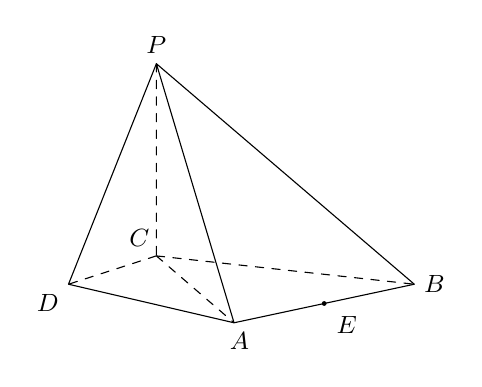
\begin{tikzpicture}[line cap=round,line join=round,font=\small,scale=0.72]
\coordinate (P) at (1.60,4.60);
\coordinate (C) at (1.60,1.21);
\coordinate (D) at (0.05,0.71);
\coordinate (B) at (6.15,0.71);
\coordinate (A) at (2.97,0.03);
\coordinate (E) at (4.56,0.37);
% 虚线先画（含 PC 竖线与底面后侧棱、对角线 CA）
\draw[dashed] (P)--(C) (C)--(D) (C)--(B) (C)--(A);
% 实线后画（压住虚线交叉处，与原图一致）
\draw (P)--(D) (P)--(B) (P)--(A) (D)--(A) (A)--(B);
\node[above] at (P) {$P$};
\node[above left,xshift=1pt] at (C) {$C$};
\node[below left] at (D) {$D$};
\node[right] at (B) {$B$};
\node[below,xshift=2pt] at (A) {$A$};
\fill (E) circle (1.2pt) node[below right,xshift=1pt,yshift=-1pt] {$E$};
\end{tikzpicture}
\end{center}
\nopagebreak[4]
（1） 求证：\(DC\perp\) 平面 \(PAC\)；

（2） 求证：平面 \(PAB\perp\) 平面 \(PAC\)；

（3） 设点 \(E\) 为 \(AB\) 的中点。在棱 \(PB\) 上是否存在点 \(F\)，使得 \(PA\parallel\) 平面 \(CEF\)？说明理由。

\Needspace{4\baselineskip}
\textbf{解析}

\gksubpart{(1)}

由 \(PC\perp\) 平面 \(ABCD\)，而 \(DC\subset\) 平面 \(ABCD\)，得 \(DC\perp PC\)。又已知 \(DC\perp AC\)，且 \(AC\) 与 \(PC\) 是平面 \(PAC\) 内交于 \(C\) 的两条直线，由线面垂直的判定定理得 \(DC\perp\) 平面 \(PAC\)。

\gksubpart{(2)}

由 (1) 得 \(DC\perp\) 平面 \(PAC\)，又 \(AB\parallel DC\)，故 \(AB\perp\) 平面 \(PAC\)。而 \(AB\subset\) 平面 \(PAB\)，由面面垂直的判定定理，平面 \(PAB\perp\) 平面 \(PAC\)。

\Needspace{14\baselineskip}

\gksubpart{(3)}

存在，\(F\) 为棱 \(PB\) 的中点。

\textbf{存在性}：取 \(F\) 为 \(PB\) 的中点。在 \(\triangle PAB\) 中，\(E\)、\(F\) 分别是 \(AB\)、\(PB\) 的中点，故 \(EF\parallel PA\)。又 \(F\notin\) 平面 \(ABCD\)（直线 \(PB\) 与平面 \(ABCD\) 只交于 \(B\)），故平面 \(CEF\neq\) 平面 \(ABCD\)，且平面 \(CEF\) 与平面 \(ABCD\) 的交线为 \(CE\)；而 \(A\notin CE\)（否则由 \(AB\perp AC\) 与 \(E\in AB\) 将导出 \(C\in AB\)，与 \(C\notin AB\) 矛盾），即 \(A\notin\) 平面 \(CEF\)，从而 \(PA\not\subset\) 平面 \(CEF\)。由线面平行的判定定理，\(PA\parallel\) 平面 \(CEF\)。

\textbf{唯一性}：设 \(F\in PB\) 且 \(PA\parallel\) 平面 \(CEF\)。由平面 \(CEF\) 与平面 \(PAB\) 的交线为 \(EF\)（\(C\notin\) 平面 \(PAB\)），及「若一条直线平行于一个平面，则过该直线的平面与此平面的交线与该直线平行」，得 \(EF\parallel PA\)。于是在 \(\triangle PAB\) 中 \(E\) 为 \(AB\) 中点且 \(EF\parallel PA\)，故 \(F\) 为 \(PB\) 的中点。所以这样的点 \(F\) 存在且唯一。

\gkanswer{答案（1）：见解析版}

\gkanswer{答案（2）：见解析版}

\gkanswer{答案（3）：存在，\(F\) 为棱 \(PB\) 的中点。}

\end{answer}
\begin{answer}
\gksolhead{19}{}

\textbf{题目}：

已知椭圆：\(C:\dfrac{x^{2}}{a^{2}}+\dfrac{y^{2}}{b^{2}}=1\) 过点 \(A(2,0)\)，\(B(0,1)\) 两点。

（1） 求椭圆 \(C\) 的方程及离心率；

（2） 设 \(P\) 为第三象限内一点且在椭圆 \(C\) 上，直线 \(PA\) 与 \(y\) 轴交于点 \(M\)，直线 \(PB\) 与 \(x\) 轴交于点 \(N\)，求证：四边形 \(ABNM\) 的面积为定值。

\Needspace{4\baselineskip}
\textbf{解析}

\gksubpart{(1)}

\Needspace{5\baselineskip}
点 \(A(2,0)\) 在椭圆上给出 \(\dfrac{4}{a^{2}}=1\)，即 \(a^{2}=4\)；点 \(B(0,1)\) 给出 \(\dfrac{1}{b^{2}}=1\)，即 \(b^{2}=1\)。故

\nopagebreak[4]
\[
C:\ \frac{x^{2}}{4}+y^{2}=1,
\]

半焦距 \(c=\sqrt{a^{2}-b^{2}}=\sqrt{3}\)，离心率 \(e=\dfrac{c}{a}=\dfrac{\sqrt{3}}{2}\)。

\gksubpart{(2)}

\Needspace{5\baselineskip}
设 \(P(x_0,y_0)\)，由 \(P\) 在第三象限得 \(x_0<0\)，\(y_0<0\)，且

\nopagebreak[4]
\[
x_0^{2}+4y_0^{2}=4. \tag{$\star$}
\]

\Needspace{5\baselineskip}
直线 \(PA\) 过 \(A(2,0)\)、\(P(x_0,y_0)\)，其在 \(y\) 轴上的截距为

\nopagebreak[4]
\[
m=\frac{2y_0}{2-x_0}<0,\qquad M(0,m);
\]

\Needspace{5\baselineskip}
直线 \(PB\) 过 \(B(0,1)\)、\(P(x_0,y_0)\)，其在 \(x\) 轴上的截距为

\nopagebreak[4]
\[
n=\frac{x_0}{1-y_0}<0,\qquad N(n,0).
\]

\Needspace{5\baselineskip}
于是 \(A\)、\(B\)、\(N\)、\(M\) 依次落在第一、二、三、四象限（含轴），按 \(A\to B\to N\to M\) 构成凸四边形，且原点在其内部，其面积等于四个三角形面积之和：

\nopagebreak[4]
\[
S=S_{\triangle OAB}+S_{\triangle OBN}+S_{\triangle ONM}+S_{\triangle OMA}
=1-\frac{n}{2}+\frac{nm}{2}-m.
\]

\Needspace{5\baselineskip}
代入 \(n=\dfrac{x_0}{1-y_0}\)、\(m=\dfrac{2y_0}{2-x_0}\)，通分（分母 \(2(1-y_0)(2-x_0)>0\)），分子为

\nopagebreak[4]
\[
2(1-y_0)(2-x_0)-x_0(2-x_0)+2x_0y_0-4y_0(1-y_0)
=4-4x_0-8y_0+4x_0y_0+(x_0^{2}+4y_0^{2}),
\]

\Needspace{5\baselineskip}
由 \((\star)\) 得分子 \(=8-4x_0-8y_0+4x_0y_0=4(1-y_0)(2-x_0)\)，故

\nopagebreak[4]
\[
S=\frac{4(1-y_0)(2-x_0)}{2(1-y_0)(2-x_0)}=2,
\]

与 \(P\) 的位置无关，为定值。

\gkanswer{答案（1）：\(\dfrac{x^{2}}{4}+y^{2}=1\)，离心率 \(e=\dfrac{\sqrt{3}}{2}\)。}

\gkanswer{答案（2）：见解析版}

\end{answer}
\begin{answer}
\gksolhead{20}{}

\textbf{题目}：

设函数 \(f(x)=x^{3}+ax^{2}+bx+c\)。

（1） 求曲线 \(y=f(x)\) 在点 \((0,f(0))\) 处的切线方程；

（2） 设 \(a=b=4\)，若函数 \(f(x)\) 有三个不同零点，求 \(c\) 的取值范围；

（3） 求证：\(a^{2}-3b>0\) 是 \(f(x)\) 有三个不同零点的必要而不充分条件。

\Needspace{4\baselineskip}
\textbf{解析}

\gksubpart{(1)}

\(f(0)=c\)，切点为 \((0,c)\)。\(f'(x)=3x^{2}+2ax+b\)，切线斜率 \(k=f'(0)=b\)，故切线方程为 \(y=bx+c\)。

\gksubpart{(2)}

\Needspace{5\baselineskip}
此时 \(f(x)=x^{3}+4x^{2}+4x+c\)，\(f'(x)=3x^{2}+8x+4=(3x+2)(x+2)\)，驻点为 \(x=-2\) 与 \(x=-\dfrac{2}{3}\)。\(f'\) 的符号为：\(x<-2\) 时正，\(-2<x<-\dfrac{2}{3}\) 时负，\(x>-\dfrac{2}{3}\) 时正，故 \(x=-2\) 处取极大值 \(f(-2)=c\)，\(x=-\dfrac{2}{3}\) 处取极小值

\nopagebreak[4]
\[
f\left(-\frac{2}{3}\right)=c-\frac{32}{27}.
\]

三次函数有三个不同零点当且仅当极大值大于零且极小值小于零（三段单调区间各含一个零点），即 \(c>0\) 且 \(c-\dfrac{32}{27}<0\)，故 \(0<c<\dfrac{32}{27}\)。（端点 \(c=0\)、\(c=\dfrac{32}{27}\) 时零点只有两个，均取不到。）

\gksubpart{(3)}

\Needspace{5\baselineskip}
\textbf{必要性}：设 \(f(x)\) 有三个不同零点 \(x_1<x_2<x_3\)。在 \([x_1,x_2]\) 与 \([x_2,x_3]\) 上分别用罗尔定理，存在 \(x_1<\xi_1<x_2<\xi_2<x_3\) 使 \(f'(\xi_1)=f'(\xi_2)=0\)，即二次函数 \(f'(x)=3x^{2}+2ax+b\) 有两个不同实根，其判别式

\nopagebreak[4]
\[
\Delta=(2a)^{2}-12b=4(a^{2}-3b)>0,
\]

故 \(a^{2}-3b>0\) 是必要的。

\textbf{不充分性}：取 \(f(x)=x^{3}+x^{2}\)（即 \(a=1\)，\(b=0\)，\(c=0\)），此时 \(a^{2}-3b=1>0\)，但 \(f(x)=x^{2}(x+1)\) 的零点为 \(x=0\)（二重）与 \(x=-1\)，只有两个不同零点。

综上，\(a^{2}-3b>0\) 是 \(f(x)\) 有三个不同零点的必要而不充分条件。

\gkanswer{答案（1）：\(y=bx+c\)。}

\gkanswer{答案（2）：\(0<c<\dfrac{32}{27}\)。}

\gkanswer{答案（3）：见解析版}

\end{answer}